\documentclass[11pt]{article}
\usepackage[utf8]{inputenc}
\usepackage[T1]{fontenc}
\usepackage{graphicx}
\usepackage[export]{adjustbox}
\graphicspath{ {./images/} }
\usepackage{amsmath}
\usepackage{amsfonts}
\usepackage{amssymb}
\usepackage[version=4]{mhchem}
\usepackage{stmaryrd}

\begin{document}
Structured Products with Exotic Option Features

The first example of a structured product in this session was the case of an insured CD that offered upside potential based on the performance of an equity index. Structured products have evolved to include highly creative and potentially highly complex investments. Many of these products use complex optionalities and often have highly sophisticated underlying valuation models.

For example, consider the following stylized description of a retail structured product that illustrates the complexity of some of these products.

This structured product provides five years of exposure to a basket of 10 underlying equities. Semiannually, the return of the best-performing equity is locked in (subject to a cap) and removed from the basket. At termination, the product pays the average of the locked-in returns of the 10 equities (subject to a floor).

What is the motivation of an investor in this product? How can an investor determine an appropriate value for the product? How can the issuer manage the risk of providing this product?

The spectrum of potential products is vast, varying on such dimensions as the number of underliers, the observation dates, floors, caps, and principal protections. Some products are sufficiently complex that their valuations depend on myriad parameters and the use of highly sophisticated Monte Carlo simulation techniques.

The starting point for understanding many complex structured products is to understand exotic options. the session, Derivatives and Risk-Neutral Valuation provides an introduction to options that emphasizes simple European-style call options and put options. A simple option has (1) payoffs based only on the value of a single underlying asset observed at the expiration date, and (2) linear payoffs to the long position of the calls and puts based on the distance between the option's strike price and the value of the underlying asset. These simple options, detailed in the session, Derivatives and Risk-Neutral Valuation, are sometimes called "plainvanilla" or "non-exotic" options. This material uses the term simple options.

Although there is no universally accepted definition of an exotic option, a useful definition is that an exotic option is an option that has one or more features that prevent it from being classified as a simple option, including payoffs based on values prior to the expiration date, and/or payoffs that are nonlinear or discontinuous functions of the underlying asset. This analysis of structured products makes the following distinction: A structured product without exotic options has a payoff diagram defined exclusively in terms of the payoff to the value of a single underlier at termination and is (1) a continuous relationship, (2) a one-to-one relationship, and (3) a relationship composed entirely of two linear segments. Thus, a structured product based on exotic options violates one or more of the three properties.

The structured products described in this session are generally engineered to the preferences of the investor. Examples are provided as a general guide to common practices in the industry. It should be noted, however, that details regarding the structured products are stylized into general conventions in this session and the illustrations provided in this session are not necessarily those found in actual products.

\section*{Structured Products with No Exotic Options}
The next exhibit is representative of a structured product that does not have exotic option features. The payout in Equivalence of Two Strategies exhibit is a simple example of a popular investment known as a principal-protected structured product. A principal-protected structured product is an investment that is engineered to provide a minimum payout guaranteed by the product's issuer (counterparty). For example, a major bank may offer a structured product with a term of five years that has a payout that increases if an underlying index increases but also a minimum guaranteed payout regardless of any declines in the underlying index. Of course, the payout is subject to the counterparty risk of the issuer. Thus, in the context of structured products, principal protection is the promise by the issuer to guarantee the return of most or all of the investor's principal.

\begin{center}
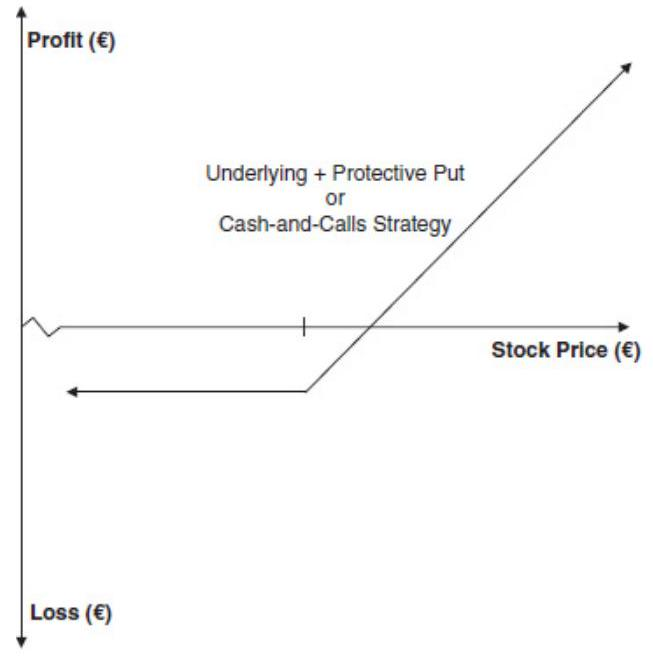
\includegraphics[max width=\textwidth]{2024_04_10_71ad1a12f130097be485g-2}
\end{center}

\section*{Equivalence of Two Strategies}
Another important feature of many structured products is the participation rate. The participation rate indicates the ratio of the product's payout to the value of the underlying asset. A structured product with a participation rate of $100 \%$ has a payout that increases by the same percentage that the underlying asset's value increases. A participation rate of $50 \%$ indicates half the risk exposure, whereas a participation rate above $100 \%$ indicates leveraged exposure of the structured product to the value of the underlying asset.

Note that principal protection and participation rates are not exotic option features. Simple call options and put options can easily be combined to provide principal protection (e.g., long a put option) and participation rates not equal to $100 \%$ (e.g., having option exposures with notional amounts above or below the principal amount of the structured product).

The diagram in the Equivalence of Two Strategies exhibit can be constructed with a long exposure to an underlying asset and a protective put. The structured product in Equivalence of Two Strategies exhibit is easy to understand and easy to value since valuation of simple options is quite easy.

The exposure illustrated in the above exhibit can also be viewed as a cash-and-call strategy. A cash-and-call strategy is a long position in cash, or a zero-coupon bond, combined with a long position in a call option. The identity between a protective put strategy and a cash-and-call strategy is a straightforward implication of put-call parity, as discussed in the session, Derivatives and Risk-Neutral Valuation. Thus, prices of the components of a structured product may often be related based on the put-call parity relationship.

The structured product depicted in Equivalence of Two Strategies exhibit may be viewed and valued quite simply using simple options. However, the payoffs in Binary Call Options and Up-and-In Barrier Call Option exhibits contain exotic options, some of which may be very difficult to price.

\begin{center}
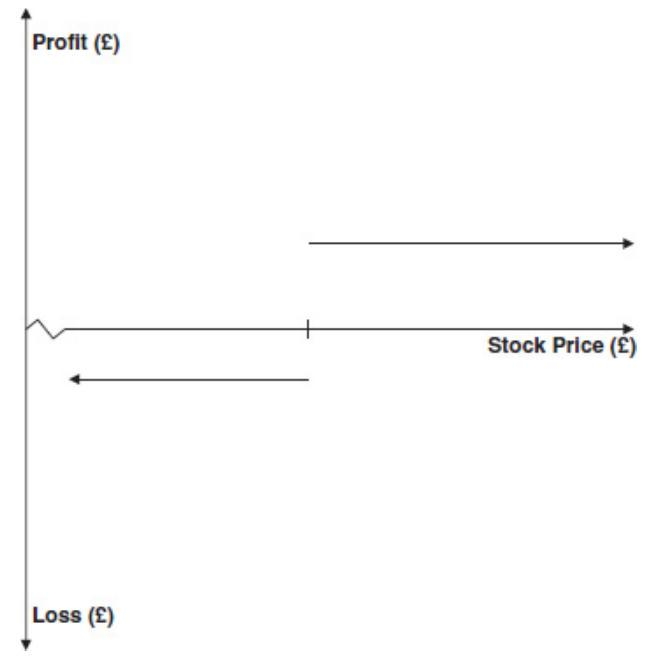
\includegraphics[max width=\textwidth]{2024_04_10_71ad1a12f130097be485g-3}
\end{center}

\section*{Binary Call Options}
\begin{center}
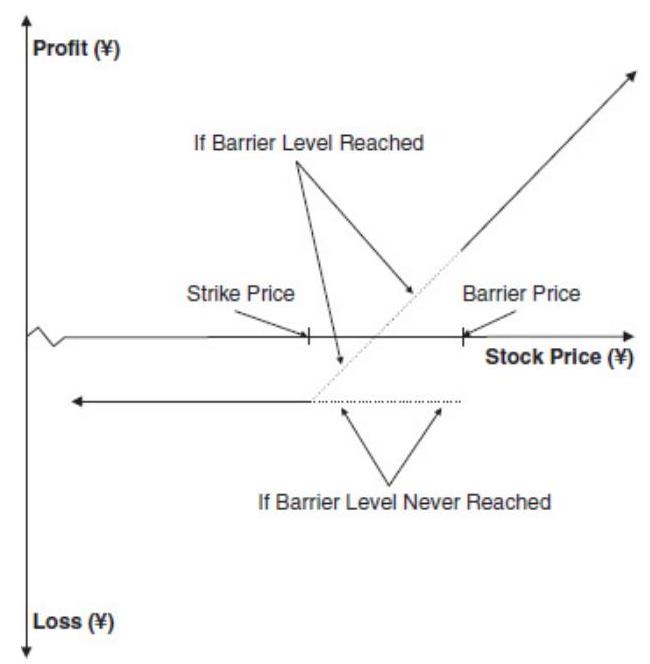
\includegraphics[max width=\textwidth]{2024_04_10_71ad1a12f130097be485g-3(1)}
\end{center}

Up-and-In Barrier Call Option

\section*{Structured Products and Asian Options}
Some options have payoffs that depend on market values at multiple points in time. An Asian option is an option with a payoff that depends on the average price of an underlying asset through time.

Consider an Asian call option on oil prices that pays the greater of $X$ - K or zero, where $X$ is the average market price of the underlying asset observed monthly over a one-year period and $K$ is the strike price. A firm that uses oil every month can purchase this single option and, in so doing, can cap its average oil costs over the 12\\
months. The purchase of one Asian option is less expensive than the purchase of 12 monthly European options because it offers less protection. However, the protection offered by the Asian option might better fit the firm's desire to lock in a maximum average annual price of the oil purchases.

A path-dependent option is any option with a payoff that depends on the value of the underlying asset at points prior to the option's expiration date. An American option is a path-dependent option because the payoff from the option writer to the option holder can be affected by the values of the underlying asset prior to the option's expiration.

There are other options discussed in later sections, such as path-dependent options, that are more complex than Asian options. Note that just because an option has an average price as an underlier does not necessarily mean that the option should be characterized as an Asian option. The averaging process in an Asian option should be based on averaging prices through time. An option on the average price of two or more underlying assets at the same point in time does not typically qualify as an Asian option. For example, an option on the average (non-annualized) return of 10 securities is not an Asian option; it is an option on a portfolio.

\section*{Structured Products and Binary Options}
Binary options were introduced in the session, Credit Risk and Credit Derivatives in the context of credit derivatives. In the case of credit options, a binary option provides two payoffs, contingent on whether a specified credit event occurs at any point in time over the life of the option.

The binary options in the structured products in this session are European options and are a little different. A binary option in a structured product has two potential payoffs, based on whether the value of the underlying asset is above or below the binary option's strike price at the option's expiration (i.e., at the termination of the structured product).

Binary Call Options illustrates the upward jump in the payoff of a binary call option that occurs when the underlying asset's price exceeds the call option's strike price at the termination of the product. The diagram is discontinuous and is based solely on the final price of the underlier, as illustrated in Binary Call Options. The discontinuous jump in the option price relative to the price of the underlying asset at the termination of the product is the key feature of a binary option. Other types of structured products or options, discussed later, offer large price jumps, but they do so either with multiple payoff levels or based on prices other than the price of the underlier at the termination of the product.

\section*{Structured Products and Barrier Options}
Barrier options are a type of path-dependent option. Structured products often include barrier options. A barrier option is an option in which a change in the payoff is triggered if the underlying asset reaches a prespecified level during a prespecified time period. For example, a structured product that permanently loses principal protection if the underlying asset reaches a specified loss level contains a barrier option.

Barrier option features are either knock-in options or knock-out options. A knock-in option is an option that becomes active if and only if the underlying asset reaches a prespecified barrier. An active option in a barrier option is an option for which the underlying asset has reached the barrier and is therefore triggered as being in effect. Once a barrier option has become an active option, the option can affect the payoff without further need for the underlying asset to reach the barrier again. If the underlying asset price never reaches the barrier, then the option remains inactive and expires worthless. Knock-in options can be calls or puts, depending on whether it is a call or put that becomes active.

For example, consider a knock-in call option on an asset with a current price of $\$ 100$ and a barrier of $\$ 110$. If the underlying asset moves up and reaches the barrier (\$110), the option becomes a simple active call option. Further, suppose that the option's strike price is $\$ 105$. If the price of the underlying asset never reaches the barrier ( $\$ 110$ ), the option expires worthless. Thus, even if the underlying asset reaches $\$ 109$ prior to expiration, the option holder receives no payoff if the $\$ 110$ level was never reached. Once the barrier has been reached, the option will behave like a simple option with a payoff that is determined solely by the relationship between the price of the underlying asset and the strike price.

\section*{Characteristics of In versus Out and Up versus Down Barrier Options}
The option described in the preceding section is a type of knock-in option known as an up-and-in call option. It is an "up" option because the price of the underlying asset is less than the barrier price at inception, and therefore the underlying asset must move up in price for the option to have value. It is an "in" option because the option becomes active if the barrier is reached. It is a call option because the option that can become active is a call option.

A knock-out option is an option that becomes inactive (i.e., terminates) if and only if the underlying asset reaches a prespecified barrier. If the underlying asset price never reaches the barrier, then the option remains active and can be exercised at expiration. Knock-out options can be calls or puts and be issued as up or down options.

Barrier Calls and Puts depicts eight types of options differentiated by being up/down, in/out, or call/put. The up-and-in call option is depicted in the upper left corner.

Barrier Calls and Puts

\begin{center}
\begin{tabular}{lll}
 & Barrier > Underlier & Barrier < Underlier \\
\hline
Knock-in & Up-and-in call or put & Down-and-in call or put \\
Knock-out & Up-and-out call or put & Down-and-out call or put \\
\hline
\end{tabular}
\end{center}

In the lower right corner of Barrier Calls and Puts is a type of knock-out option known as a down-and-out put. A down-and-out put becomes inactive if the price of the underlying asset falls to the barrier. Thus, the payoff of the put is limited to the excess of the strike price $(K)$ above the barrier ( $H$ ). It is a "down" option because the price of the underlying asset is greater than the barrier price at inception, and, therefore, the underlying asset must move down in price to reach the barrier. It is an "out" option because the option becomes inactive if the barrier is reached. It is a put option because the option that can become inactive is a put option.

Note that a down-and-out put is not the same as a simple put option spread that is long a put with a strike price of $K$ and short a put with a strike price of $H$ (with $K>$ $H)$. The reason is that at expiration, the put spread will pay the greater of $K-H$ or zero. However, the down-and-out put will pay $K-H$ only if the barrier is never reached. If the barrier is reached at any time prior to expiration of the knock-out feature, the barrier put pays nothing.

Note that barrier options should always have values equal to or less than simple options of the same maturity and strike price, as barrier options can have the potential for an earlier expiration and lower payoff.

The Up-and-In Barrier Call Option exhibit illustrates the payoff diagram of a barrier option. Notice that the payoff is no longer purely a function of the value of the underlier at option expiration. Over some of the range, the payoff to the option can take on one of two values depending on the path that the underlier took. Specifically, one path is based on the underlier not having reached the barrier, and the other is based on the underlier having reached the barrier.

Structured products with path-dependent options tend to have complex payout diagrams that capture the paths through multiple payout lines based on conditions related to the paths, as shown in the exhibit, Up-and-In Barrier Call Option.

\section*{Structured Products and Spread Options}
A spread option has a payoff that depends on the difference between two prices or two rates, such as the price (or rate) of asset \#1 minus the price (or rate) of asset \#2. The option's payoff is the greater of zero and the underlying spread less the option's strike price (or strike rate) at expiration. Note: A spread option should not be confused with option spreads, discussed in the session, Derivatives and Risk-Neutral Valuation, which are portfolios with multiple call or put positions.

Consider, for example, a one-year European spread call option with a strike price (or strike rate) of $2 \%$ on the difference of the percentage return of a large-cap equity index over the percentage return of a small-cap equity index. Assume that at the end of the year, the large-cap index has risen $10 \%$ and the small-cap index has risen $4 \%$. Accordingly, the spread between the returns is $+6 \%$. A spread call with a strike price of $2 \%$ would pay $4 \%$ (of the option's notional value) to its holder. A call spread option pays its holder when the spread exceeds the strike, whereas a put spread option pays its holder when the spread is less than the strike. A spread put with a strike price of $2 \%$ in this example would expire worthless.

Note that the spread between two assets may be represented as either asset \#1 minus asset \#2 or the reverse, asset \#2 minus asset \#1. A call spread with a strike of $K$ is identical to a put spread with a strike of $-K$ if the definition of the spread on the put is the reverse of the definition of the spread on the call.

\section*{Structured Products and Look-Back Options}
Another type of path-dependent option is a look-back option. A look-back option has a payoff based on a minimum or maximum price that occurs over a specified period of time (the look-back period). Typically, the look-back period is the entire life of the option. An in-the-money look-back call pays the maximum price over the look-back period minus the strike price. An in-the-money look-back put pays the strike price minus the minimum price over the look-back period.

\section*{Quantos and Other Structured Products}
The spectrum of structured products provided by issuers throughout the world to meet investor preferences is astounding. An example of a very specialized option is a quanto. A quanto option is an option with a payoff based in one currency using the numerical value of the underlying asset expressed in a different currency. For example, the Nikkei 225 is a yen-based index of Japanese stock prices. Consider a U.S. dollar-based quanto call option on the Nikkei with a strike price of 17,000 issued when the Nikkei 225 was at 16,000 . This quanto call option on the Nikkei 225 would pay $\$ 1$ for every point by which the Nikkei 225 exceeded 17,000 at the option's expiration.

The preceding discussions have covered some of the major categories of exotic options used in structured products, but other option-driven products exist. For example, some advanced structured products have payouts that depend on the prices of a set of underlying assets. The payouts to these structured products can involve valuations at a variety of points in time (e.g., quarterly over the product's life), resulting in payouts related to some of the underlying asset values being capped or frozen at each valuation point, and payouts related to the remaining underlying assets being allowed to continue to vary until the option's expiration.


\end{document}